\documentclass[10pt,twocolumn,letterpaper]{article}

\usepackage{cvpr}
\usepackage{times}
\usepackage{epsfig}
\usepackage{graphicx}
\usepackage{amsmath}
\usepackage{amssymb}


% Include other packages here, before hyperref.

% If you comment hyperref and then uncomment it, you should delete
% egpaper.aux before re-running latex.  (Or just hit 'q' on the first latex
% run, let it finish, and you should be clear).
\usepackage[breaklinks=true,bookmarks=false]{hyperref}

\cvprfinalcopy % *** Uncomment this line for the final submission

\def\cvprPaperID{****} % *** Enter the CVPR Paper ID here
\def\httilde{\mbox{\tt\raisebox{-.5ex}{\symbol{126}}}}

\renewcommand{\arraystretch}{1.4}

% Pages are numbered in submission mode, and unnumbered in camera-ready
%\ifcvprfinal\pagestyle{empty}\fi
\setcounter{page}{1}
\begin{document}

%%%%%%%%% TITLE
\title{Hierarchical Multiclass Object Classification }

\author{Fereshte Khani\\ 
Massachusetts Institute of Technology\\
{\tt\small fereshte@mit.edu}
% For a paper whose authors are all at the same institution,
% omit the following lines up until the closing ``}''.
% Additional authors and addresses can be added with ``\and'',
% just like the second author.
% To save space, use either the email address or home page, not both
\and
Anurag Mukkara\\
Massachusetts Institute of Technology\\
{\tt\small anurag\_m@mit.edu}
}

% TODO
% spell check
% bold text for variables


\maketitle
%\thispagestyle{empty}

%%%%%%%%% ABSTRACT
\begin{abstract}
	
	Human can use similarity between objects in order to recognize rare objects. They also make many abstract concepts when they see some objects very often. Interestingly, a large part of brain is associated with common classes like faces rather than rare objects like Ostrich.
	In our work we want to propose a model that has four mentioned characteristics.1. Use more resources for categories that have many examples and less resources for categories that have few examples, 2. Has the ability recognize objects that it has never seen before, but can be made by combining previously seen objects, 3. Objects with few examples can borrow statistical strength from similar objects with many examples, 4. Models that have lot of sharing between model parameters of different classes should be favored.
	
\end{abstract}

%%%%%%%%% BODY TEXT
\section{Introduction}

Object classification is one of the fundamental problem in computer vision it is more harder when number of categories is large. When number of categories is very large the complexity of the model should not be related to the number of categories. It should capture the similarities between categories in order to classify objects easier and more accurate.

we all have a hierarchical based abstract concepts for object around us. We make more hierarchical concepts for object that we encounter more often. For example, if you ask a person about furniture they can categorized it by chair, desk, sofa, table, etc. and then for chair it goes like office chair, armchair, rock chair, or even wheelchair. However, we call all parrots, just parrots while there are 372 species of them.

These sub categories are related to each other visually. In this work we try to propose a model that makes more abstract concepts when there are lots of similar classes and less otherwise. This model also share many parameters between similar objects. It helps rare object that we have less training example from them use parameters of common examples. In other words, common classes have lots of training example and by them algorithm can set accurate parameters. In other hand, rare objects have very few examples and setting the parameters in an accurate way is almost impossible . Sharing parameters between these classes help rare classes to borrow statistical strength from common classes. 

We all make a model for every concept and when encounter a new object we try to check to which concept model it matches more. All learning algorithm try to add additional information to the problem to avoid over fitting. They usually use Occam-razor to have models as simple as possible. Here we want to change this regularization in a way that if a model use previously learned objects it can have more complex shape. By this structure Models that have lot of sharing between model parameters of different classes will be favored.

There are many objects around us. In the model that we have many categories, when we want to train a classifier to learn objects we should be able to model the similarities between different categories otherwise we should store many redundant information. In one vs all methods there is no difference between bicycle vs motorcycle and dogs vs motorcycle. While we like that if we have a false positive for motorcycle it should be bicycle rather than dogs. Even human sometime confused between different dogs or wrongly assume another animal to be a dog. So, we want a classifier to model this similarities.  

The rest of paper is as follows, in section two we overview the related works. There is an overview about independent classifier methods in section three. In section four we explain our method which is hierarchical multi-class model for object recognition. Finally, there is experiment in section four and Conclusion and Future works come in section five.


\section{Related works}

There are lots of work being done in the transfer learning in object classification. There are three main questions that people should answer when they want to use transfer learning. 1) What to transfer?,  2) How to transfer?, When to transfer?. For a good survey in transfer learning see \cite{transfersurvey}

For the first questions, they are methods that share parameters between classes like you can learn parameter of deep network \cite{deepnetwork} by Imagenet \cite{imagenet} and then test it in another benchmark. Some methods share training examples between classes \cite{semi}. Some share attributes \cite{attributes} and so on.

One important aspect of second question is between which classes we should transfer parameters/features. For example when we add a new class we should decide that with which classes this class should share features. Consider that we just have a few example from each class so deciding which classes should share information and which classes should not is a hard question.

For fining which classes should share information some method use a global priori \cite{priori} (share information between all classes) which provides small benefits but still is better than independent classifiers. There are some models \cite{semantic} that use external hierarchy. As an example in \cite{semantic} wordnet \cite{wordnet} is a semantic network for english language. Words are grouped together if they are synonyms and record semantic relation between them. With this dictionary one can understand both bicycle and care belong to vehicle.

Ruslan et all. \cite{ruslan}  make a tree in which every class is a leaf. In their setting height of tree is fixed and is equal to two. However, number of nodes in the tree is not fixed and they use CRP to decide if they should add another node to the tree or not. Classes which have common parent share features. They add classes incrementally to the tree. At each step they decide where in the tree they should put the class. Although this setting support feature 3, it does not the other features mentioned before. Ruslan improve his work on \cite{ruslan2} with deep network features.

Sivic et all \cite{sivic} group images using multi-layer hierarchy tree. Tree is based on common visual elements. They used generative Hierarchical Latent Dirichlet Allocation(hLDA). This model usually use for unsupervised of topic hierarchies. In this work they automatically (without supervision) discover a hierarchical structure for the visual world using unlabeled images. They are also some model that try to find some relation between categories and use them to classify images \cite{transfer22}.

For the last question that when we should transfer, algorithms deal with questions like this: should we use transfer information just for testing or we can use them for training as well? If we want to use transfer information during learning should we use them at first or in the middle? Another main issue in this area is that when it is good to transfer information, and when it make it worse when we transfer information. See \cite{whentransfer} for more details.

%In \cite{wordnet} 
%There are papers that use hierarchical for sharing features and parameters between classifiers. f
%There are many algorithms in the field of transfer learning in multi class object %recognition.(\cite{miller2000learning}) 


\section{Hierarchical Classification Model}

\subsection{Learning Independent Classification Models}

Consider a classification problem where we observe a dataset $D$ of labelled  training examples. 
Each example belongs belongs to one $K$ classes(eg. 40 object categories). The dataset $D$
has $n_{k}$ labeled examples for for each class $k  \in {1,2,....,K} $. We $x_{i}^{(k)} \in R^{D} $ 
be the input feature vector of length D for the $i^{th}$ training example of class $k$ and 
$y_{i}^{(k)}$ be the corresponding class label. $ y_{i}^{k} = 1 $ indicates that the $i^{th}$ training example 
 is a positive example for class $K$ and  $ y_{i}^{k} = -1 $ indicates that the $i^{th}$ training example 
 is a negative example for class $K$.
 
 For a binary classification problem we can use a simple logistic regression model. In particular, 
 for each class $k$, the probability of a positive instance can be modeled as: 
 \begin{equation}
 p(y_{i}^{(k)} = 1 | \beta^{(k)} )  = \frac { \exp( \beta^{(k)^{T}}  x_{i}^{(k)})  }{  1 + \exp(\beta^{(k)^{T}}  x_{i}^{(k)} ) } 
 \end{equation}
  where $k$ ranges over the $K$ classes and $ \beta^{k}  \in R^{D} $ is the unknown model parameter of length D 
  for class k. 
  In addition, we place a zero-mean spherical Gaussian prior over each model parameter  $  \beta^{k} $:
  \begin{equation}
	p(\beta)  = \prod_{k=1}^{K} p(\beta^{(k)}) = \prod_{k=1}^{K} N(0, \frac{1}{\lambda})
  \end{equation}
 where $N(\mu, \Sigma)$ indicates a Gaussian probability distribution with mean $\mu$ and covariance $\Sigma$.
 Here, $\lambda$ is the prior parameter.  With this modeling framework, the log posterior distribution of the unknown 
 parameters can be expresses as 
 \begin{equation}
	\log p(\beta | D) \propto \sum_{k=1}^{K} \Big[ \, \ \sum_{i=1}^{n_{k}} \log p(y_{i}^{(k)} | x_{i}^{(k)}, \beta^{(k)}) \ + \ \log p(\beta^{(k)}) \ \Big] \,
\end{equation}
 Maximizing the log posterior(or finding the MAP estimate ) over the unknown model parameters $\beta$  is  equivalent to 
 minimizing the probabilistic loss function with quadratic regularization terms:
 \begin{equation}
 	E = \sum_{k=1}^{K}  \Big[ \, \ \sum_{i=1}^{n_{k}} Loss(y_{i}^{(k)}, x_{i}^{(k)}, \beta^{(k)}) + \frac{\lambda}{2} \| \beta^{(k)}) \|^{2} \ \Big] \,
 \end{equation} 
 where the probabilistic loss function is given by:
 \begin{equation}
 %Loss(y_{i}^{(k)},  x_{i}^{(k)},  \beta^{(k)})  =  - \sum_{j \in {-1,1} } I\{y_{i}^{(k)}=j\} \log p(y_{i}^{(k)}=j | x_{i}^{(k)},\beta^{(k)})
 Loss(y,  x,  \beta)  =  - \sum_{j \in {-1,1} } I\{y=j\} \log p(y=j | x,\beta)
\end{equation} 
One important property of the loss function is that it is convex and hence can be efficiently optimized
using standard convex optimization solvers.
 
 The main drawback of this formulation is that all the $K$ classes are treated as unrelated entities and hence 
 do not share any model parameters. In fact, it is observed that the objective function decomposes into 
 $K$ sub-problems, each of which is a binary classification problem that can be trained independently 
 using the training data for that particular class.
 
 
 \subsection{Learning a Hierarchical Classification Model}
 In our framework, a hierarchical tree structure is used to model sharing of parameters between 
 visually related classes. Each node in the tree has a model parameter, a vector of length $D$ 
 associated with it.  Let $ \theta = \{ \theta_{1}, \theta_{2},.....,\theta_{n}\} $ denote the model parameters 
 of all the nodes in the tree, where $n$ is the number of nodes starting from the root node to the all the leaf nodes.
 The leaf nodes correspond to the $K$ object categories or classes. The parameters for a particular class $k$
 is the sum of the parameters of all the nodes, say $i_{1}, i_{2}, ..., i_{l} $, along the path from the leaf node
 corresponding to that class up until the root node of the tree:
 \begin{equation} \label{beta-theta-rel}
 \beta^{(k)} = \theta_{i_{1}} +  \theta_{i_{2}} + ...... + \theta_{i_{l}}
  \end{equation} 
 We place zero-mean spherical Gaussian priors on the parameters of each node. However, the 
 covariance matrix is dependent on the level of a particular node in the tree i.e all the nodes at
 a particular level have the same prior parameters.
 \begin{equation}
 p(\theta_{i})  = N(0,\frac{1}{\lambda_{l}}I) 
\end{equation}   
where node $i$ is at level $l$ in the tree. The root node has level 0 and the level increases as 
we move towards the leaf nodes.

With this modification in the way the model parameters for classes are related,  the hierarchical 
learning problem can be formulated as minimizing the log posterior or equivalently the loss function 
with respect to $\beta$:
\begin{equation} \label{hier-loss}
\begin{split}
E = Loss(Y,X,\beta) + \frac{\lambda_{0}}{2} \|\theta_{0} \|^{2} +
\sum_{i=1}^{k_{1}} \frac{\lambda_{1}}{2} \|\theta_{i1} \|^{2} & \\
+ \sum_{i=1}^{k_{2}} \frac{\lambda_{2}}{2} \|\theta_{i2} \|^{2} +
...... +
\sum_{i=1}^{k_{l}} \frac{\lambda_{l}}{2} \|\theta_{il} \|^{2} &
\end{split}
\end{equation} 
 where $Loss(Y,X,\beta)$ is the loss function as explained in the previous section
 but with the additional constraint that $\beta$ satisfies  equation \ref{beta-theta-rel} 
 according to the tree structure. Here there are $k_{j}$ nodes in level $j$ and 
 $\theta_{1j}, \theta_{2j},.....,\theta_{k_{j}j}$ are the parameters of nodes in level $j$.
\begin{figure}[t]
	\begin{center}
		%\fbox{\rule{0pt}{2in} \rule{0.9\linewidth}{0pt}}
		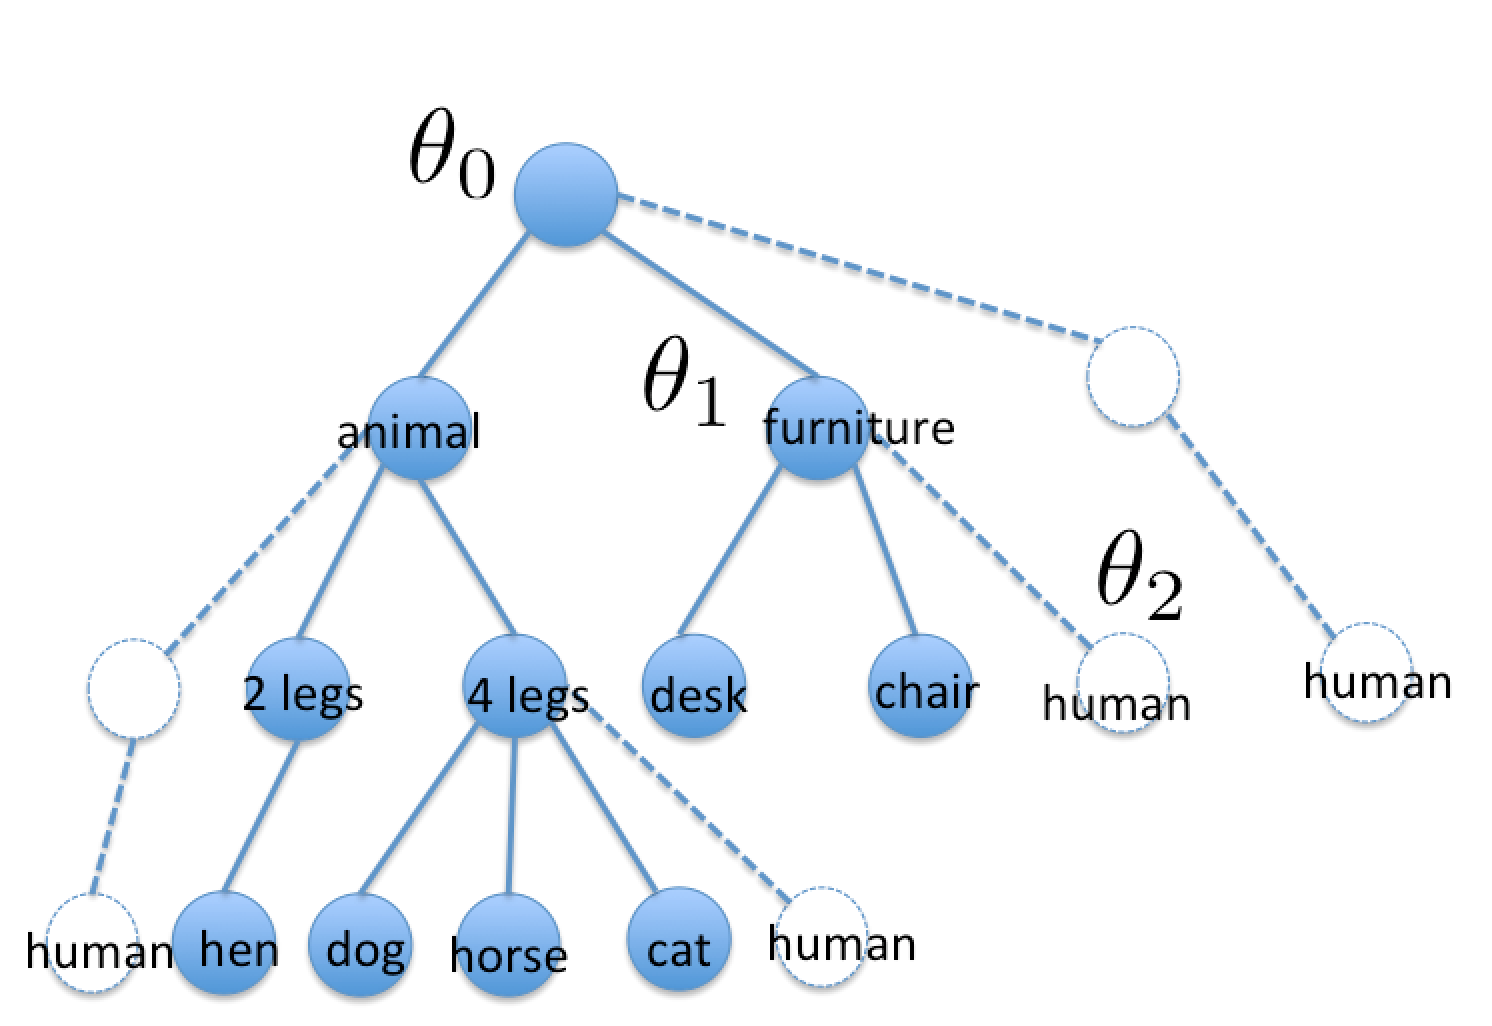
\includegraphics[width=0.8\linewidth]{tree}
	\end{center}
	\caption{Example of caption.  It is set in Roman so that mathematics
		(always set in Roman: $B \sin A = A \sin B$) may be included without an
		ugly clash.}
	\label{fig:long}
	\label{fig:onecol}
\end{figure}
\subsection{Learning the tree structure}
 \begin{figure}[t]
 	\begin{center}
 		%\fbox{\rule{0pt}{2in} \rule{0.9\linewidth}{0pt}}
 		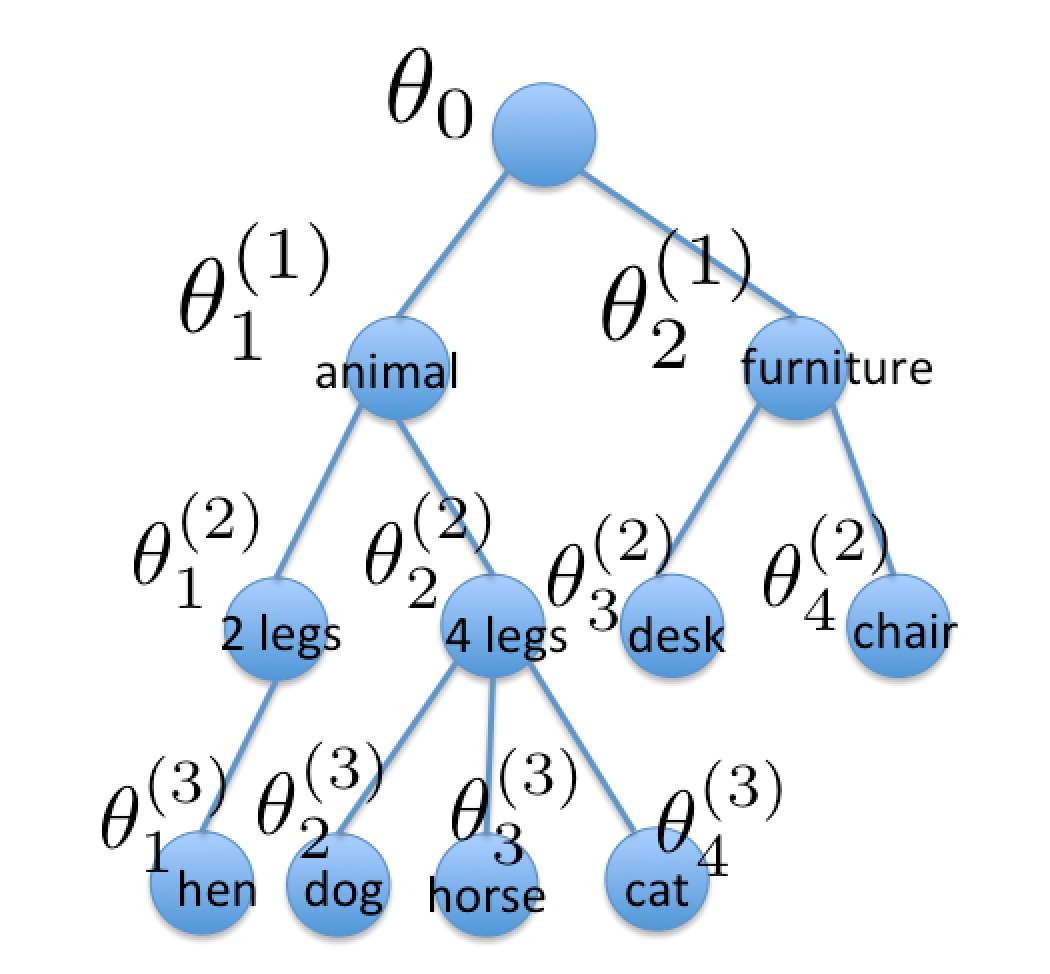
\includegraphics[width=0.8\linewidth]{tree_withoutnew}
 	\end{center}
 	\caption{Example of caption.  It is set in Roman so that mathematics
 		(always set in Roman: $B \sin A = A \sin B$) may be included without an
 		ugly clash.}
 	\label{fig:long}
 	\label{fig:onecol}
 \end{figure}
If we are given the tree structure that indicates the relation between different classes, then the 
learning algorithm only needs to optimize for the loss in equation \ref{hier-loss}. However, as 
discussed in \cite{ruslan}, learning the tree structure dynamically based on the input classes and training data
could lead to better results in object classification. We adopt the algorithm used in \cite{ruslan} to multilevel trees
and fine-grained partitioning. In \cite{ruslan}, the author use a fixed number of levels i.e 3 in the tree and use
a non-parametric Chinese Restaurant Process Prior(CRP) to model the position of a class in the tree. Although this simple
CRP prior allows one to have unknown and potentially unbounded number of groups of object classes, this is can only be
used for two-level trees. For trees which have a fixed number of levels more than 3, one could use a nested CRP prior \cite{nestedCRP}.
Since this approach has the drawback of limiting the tree to a fixed number of levels, we use a simple extension(modified-CRP) of the
CRP prior used in \cite{ruslan} to allow the flexibility of  having different depths at different parts of the tree.    

A new class could go into one of the existing super-categories or create a new super-category. A new super-category 
can be attached to any node which doesn't have any children that are leaf nodes. That is, we allow the parent of a new
super-category to be any node that is not itself a super-category that has leaf nodes, which correspond to classes, as children.
By following the procedure in \cite{ruslan},  for each possible position of the new class we calculate a likelihood term and 
modified-CRP prior term. The position of the new class will be the one that maximizes the sum of likelihood term and  prior term. 

Let $i$ denote the node number of the leaf node corresponding to the new class.   
To calculate the likelihood at a possible position in the tree, we find the model parameter $\theta_{i}$ of the leaf node, 
that maximizes the log likelihood of the training data at that position. This likelihood will depend on the position in the tree, when 
we choose a position it means that we include the parameters of all the nodes that are ancestors of the leaf node $i$ at that position. 
If the position corresponds to a category that is visually dissimilar to the new class, then the best we can with $\theta_{i}$ with still 
result in a lower likelihood term. If the the category is visually similar to the new class, we can achieve a far better fit and the likelihood
term goes up. We have observed that the maximum of the likelihood over the model parameter $\theta_{i}$ is greatly affected by the position
 we choose for the leaf node. In addition to the likelihood term, the modified-CRP prior term favors super-categories that have a large number of 
 leaf nodes or class under them. The modified-CRP prior is given by:
 
 \begin{displaymath}
 p(z=j) = \left \{
	    \begin{array}{lr}
 		\frac{m_{j}}{n+\gamma*m} & : \text{$j$ is old} \\
		\frac{\gamma}{n+\gamma*m} & : \text{$j$ is new}
	   \end{array}
	  \right.
 \end{displaymath} 
 
  \begin{figure}[t]
  	\begin{center}
  		%\fbox{\rule{0pt}{2in} \rule{0.9\linewidth}{0pt}}
  		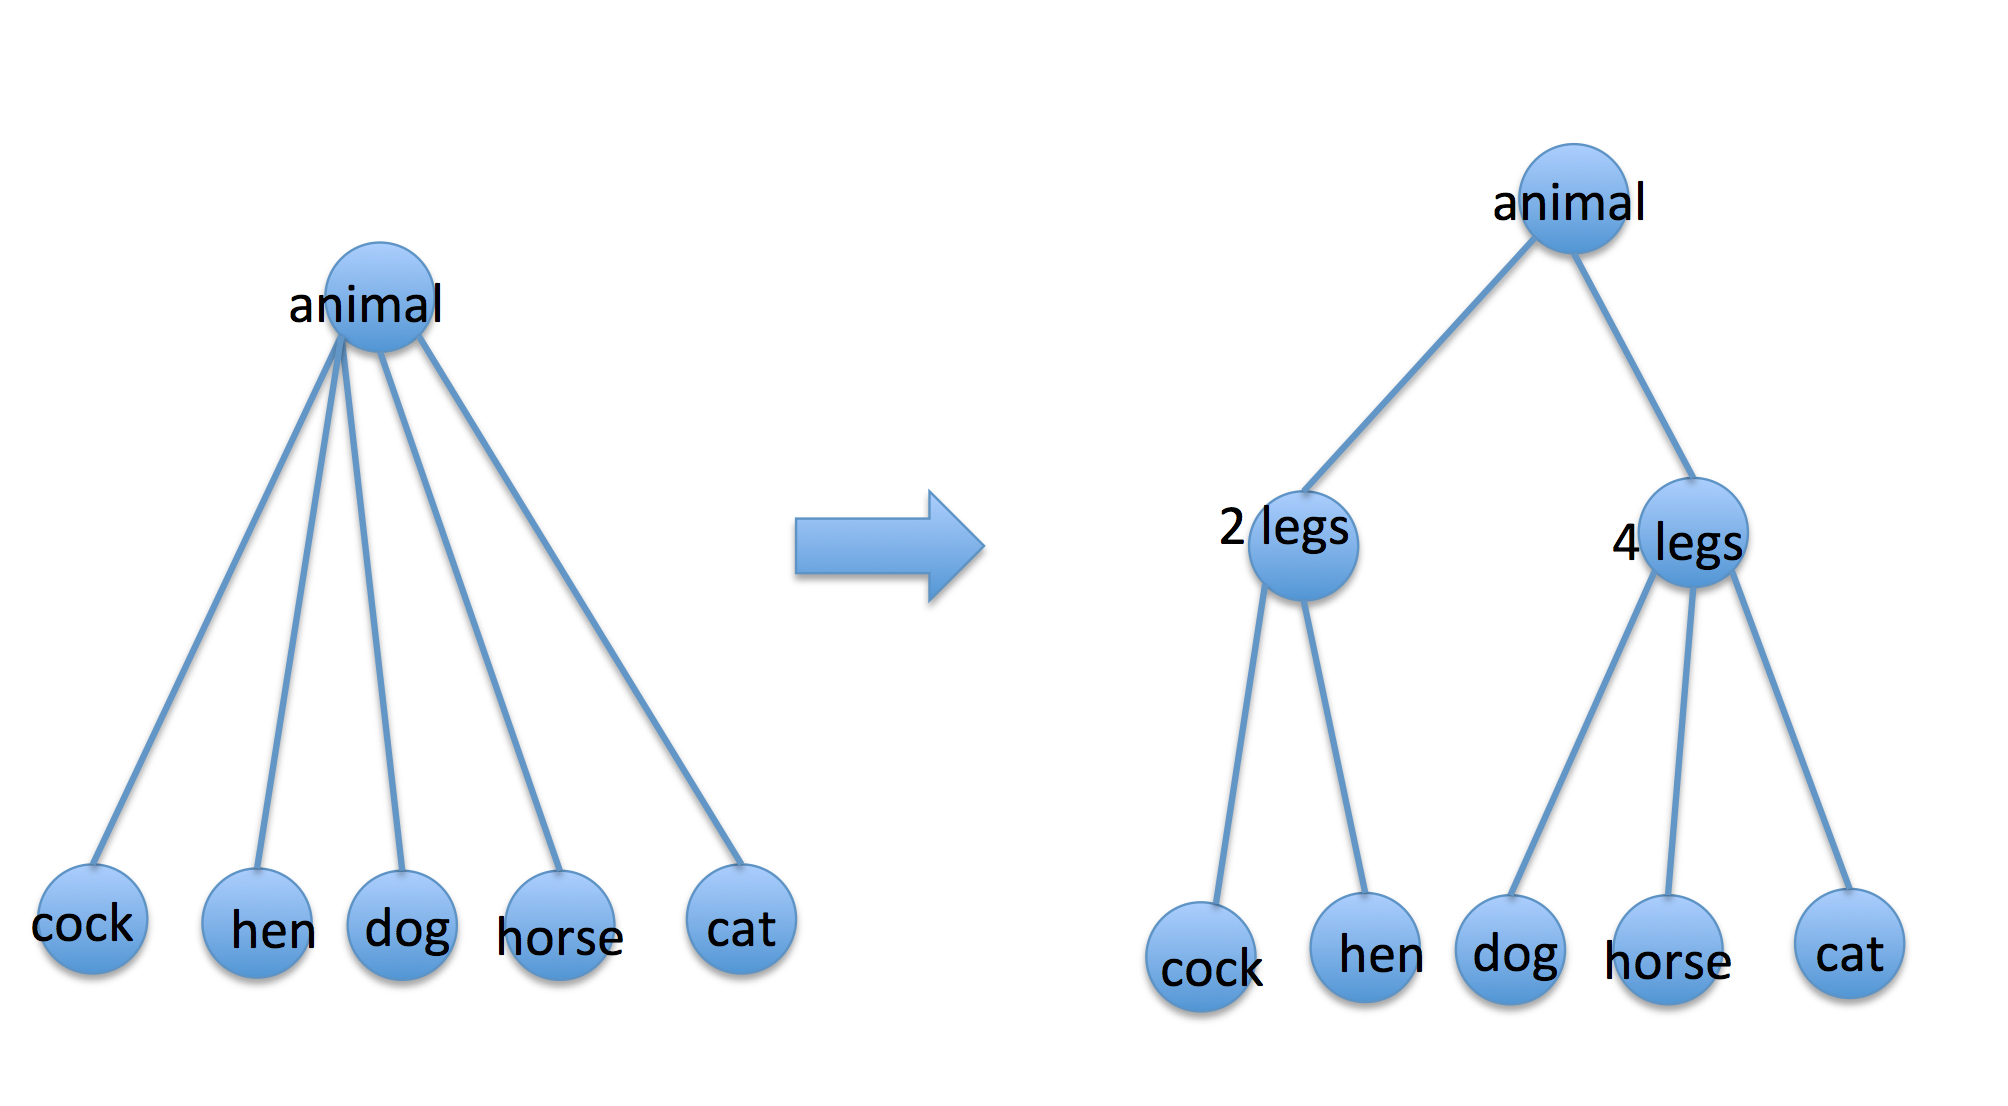
\includegraphics[width=0.8\linewidth]{split}
  	\end{center}
  	\caption{Example of caption.  It is set in Roman so that mathematics
  		(always set in Roman: $B \sin A = A \sin B$) may be included without an
  		ugly clash.}
  	\label{fig:long}
  	\label{fig:onecol}
  \end{figure}
where $n$ is the total number of leaf nodes, $m_{j}$
is the number of leaf nodes under super-category $j$,
$\gamma$ is the concentration parameter that controls the probability of creating a new super-category,
$m$ is the total number of positions of new super-categories in the tree. $m$ is equal to number of nodes
in the tree that have only super-categories as children. In other words, $m$ is the cardinality of the set that 
includes the root node as well all nodes that are not leaf nodes or parents of leaf nodes. It can be easily verified that 
this defines a valid probability distribution over the choice $z$ of possible positions in the tree where the new class can be placed.

We use same model-fitting algorithm described in \cite{ruslan} with modifications to CRP-prior term and tree structure as described above.
Basically, the algorithm alternates between deciding the position in the tree of a new class and optimizing the model parameters of all the nodes
in the tree for a given tree structure.  This alternating procedure will reach a local minima of the loss function 
described in equation \ref{hier-loss}. Since the loss function is convex, this is also the global minima of the loss function. 
For optimizing the model parameters for a fixed tree structure , we use iterative coordinate-descend procedure.
Since the parameters of all the nodes at any given level of the tree are independent of each other, we parallelize the loss minimization 
routine for these nodes. This leads to significant reduction in time taken to learn the model.

We also use a simple heuristic to maintain a fine-partitioning of the classes among into among super-categories. 
We need to avoid many leaf nodes accumulating under the 
same super-category as this would lead to a very coarse-grain partitioning of the classes.  So, whenever the number of leaf nodes under a 
super-category goes above a certain threshold $maxChild$, we break down the subtree under that node to create
 a more fine-grained partitioning.  To do this we run the entire optimization algorithm described above on the classes that were originally under this
 super-category. Basically, we consider the node corresponding to the super-category as a root node and keep adding new leaf nodes 
 to form a tree under this root node. In most cases, the $maxChild$ number of classes that previously shared the same parent are dividing
 several finer super-categories and have different parents.  In the rare case when the classes are very similar to each other, this process will add
 redundant to the tree. We identify this pathology and remove the redundant node while appropriately modifying the modle parameters of the 
 relevant nodes. The parameter $maxChild$ can be configured to control the degree of fine-grained partitioning of classes. A lower value
 of $maxChild$ leads to very fine-grained partitions whereas a higher value of $maxChild$ results in coarser partitions. We found that 
 a value of four results in best results. 
 
 \begin{figure}[t]
 	\begin{center}
 		%\fbox{\rule{0pt}{2in} \rule{0.9\linewidth}{0pt}}
 		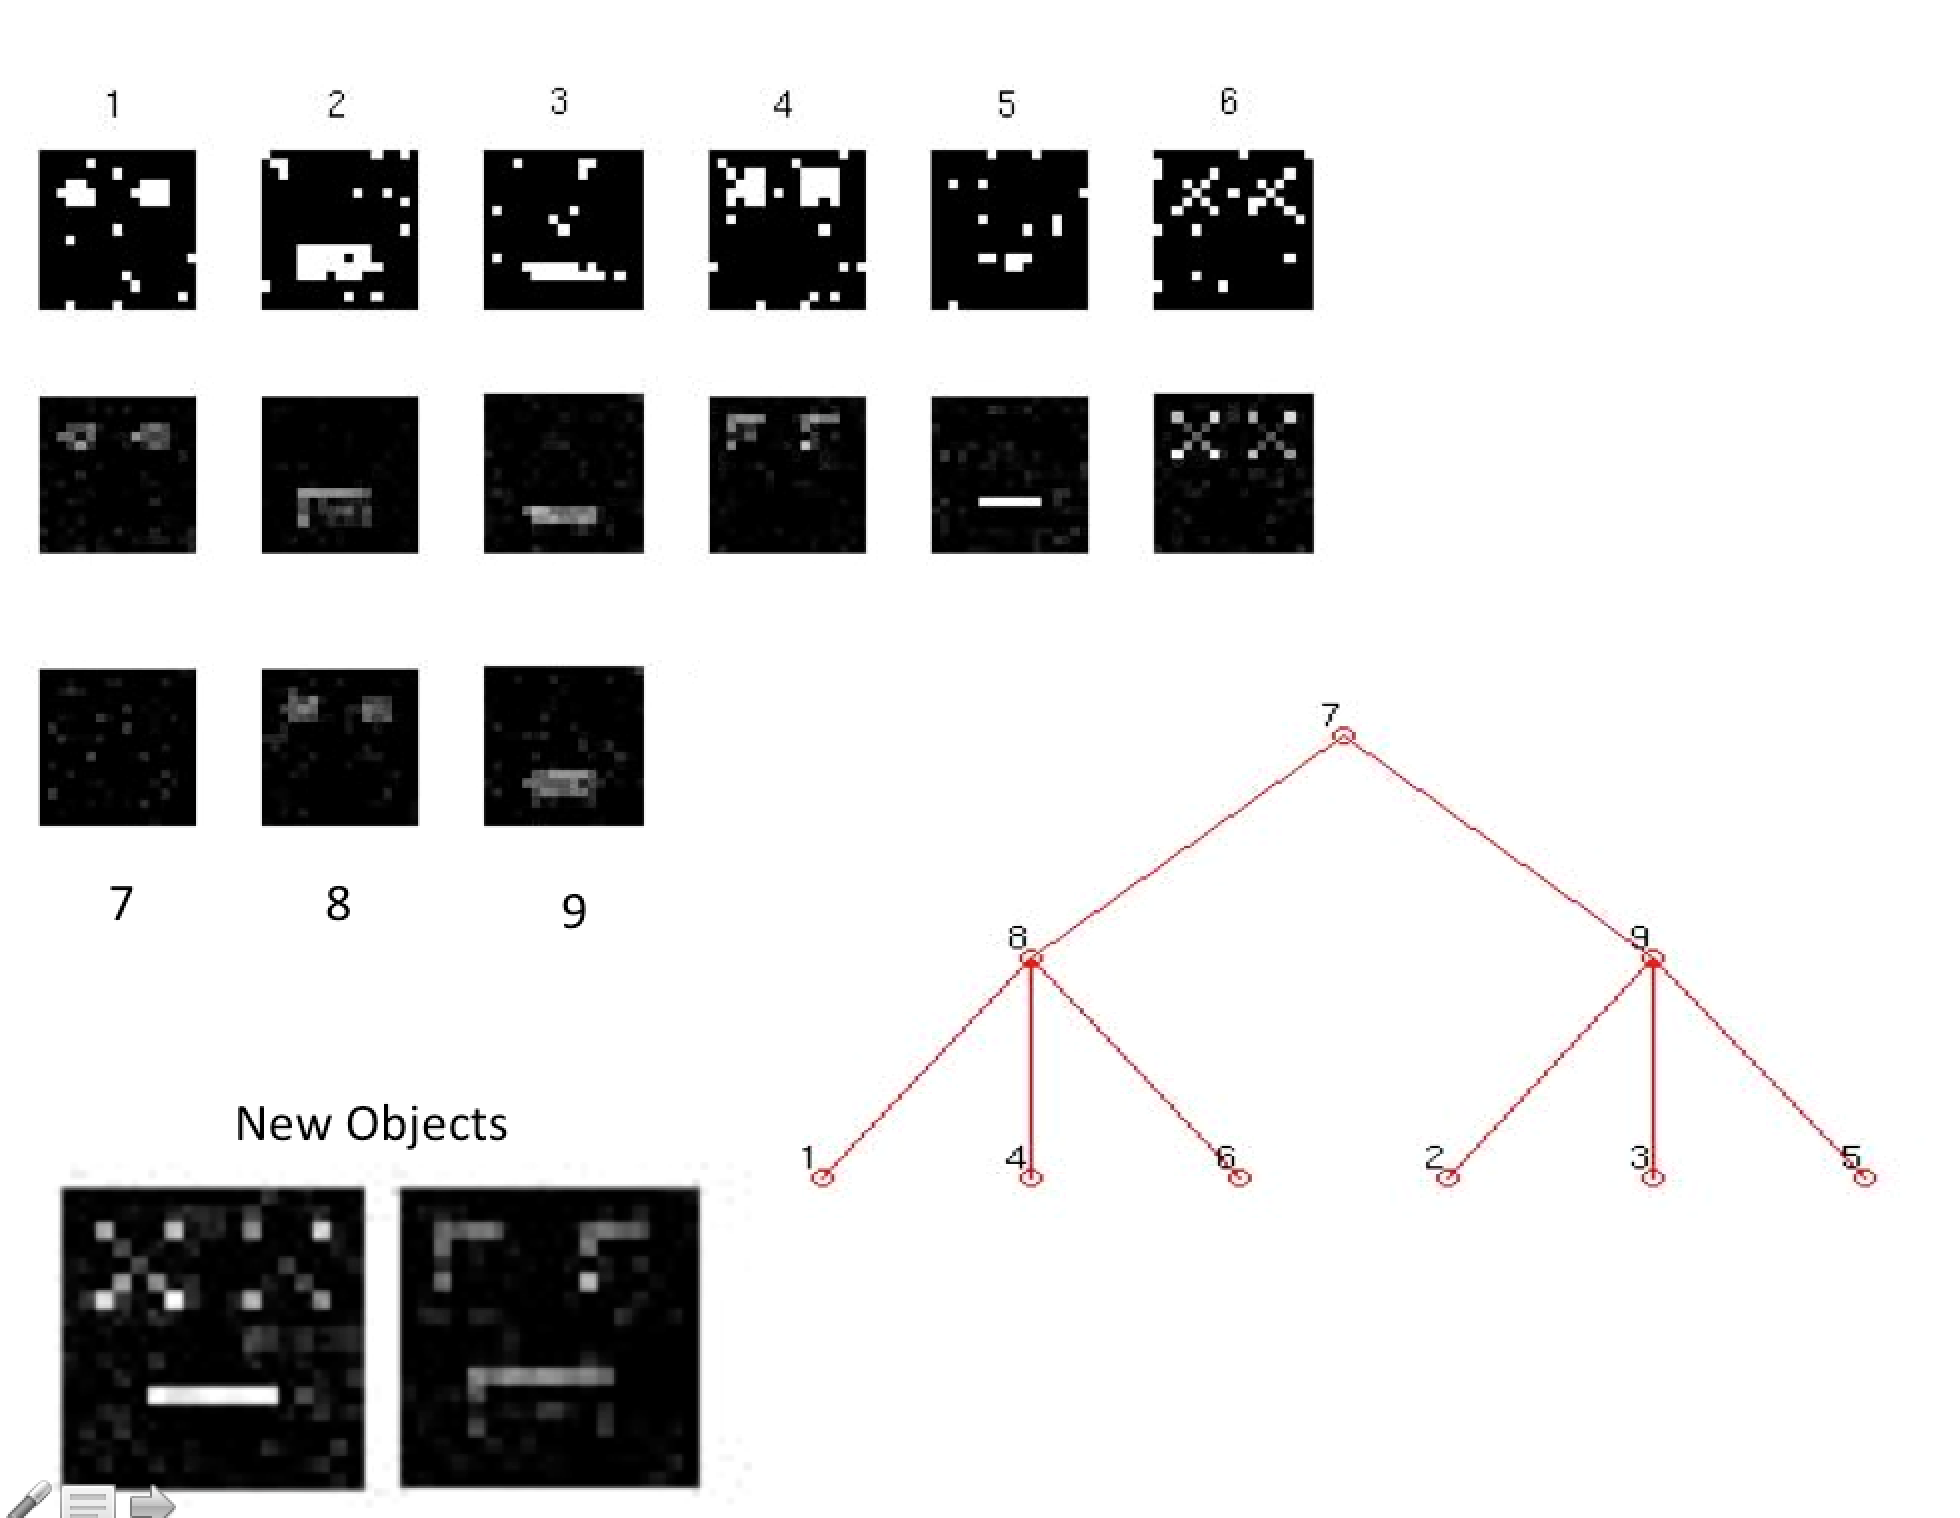
\includegraphics[width=0.8\linewidth]{smiley}
 	\end{center}
 	\caption{(a) First row shows eight classes of smiley faces. class 1,4,6 just have eys and class 2,3,5 just have eyes. The second row show the visualization for parameter $\theta$ for each node. The third line shows the visualization of $\theta$ for node 7,8,8 respectively. (b) shows the tree corossponding to these examples. As you can see in the visualization of parameter of node 7,8 they capture that there are eyes or mouthes in their children. (c) shows two visualizatoin of smiley faces by adding parameter by adding parameter $\theta$ of different nodes. If a new example which is look like these two come for testing we can identify it by these two}
 	\label{fig:smiley}
 %	\label{smiley}
 \end{figure}
\section {Experiments}
 
 \subsection {Implementation}
 We implement the whole algorithm in MATLAB the code is available in \cite{website:sourceCode}. We use Hog features for finding $\phi(x)$ for images. We use \textit{fminunc} function for optimizing our loss function.
 One can use HOGgles \cite{hoggles} in order to visualize the  abstract concepts.
 
 \subsection{Data Sets}
 \subsubsection{Smiley Faces}
 We make a syntactic data set in order to check our algorithm abilities. (merging two subcategories, make meaningful abstract concepts, make more nodes when there are more classes). There are 320 classes in this data set. Each class is a smiley face that has different nose, mouth, face and eyes. There are 1000 positive and negative examples in each classes. The pictures are 25 by 25 and we add noises added to each example of the class.
  
 \subsubsection{Fine Grained Data Set}
 We use data set of fine grained challenge \cite{dataSet}.There are five different domains (Cars, Birds, Aircrafts, Shoes and dogs) in this data set. In each domain there are about 100 classes. Classes are very similar to each other there are different type of cars, dogs and etc.
 \subsection{Results}
 \subsubsection{Smiley Faces}
 
 As mentioned before the main reason for making this dataset was to visualize our algorithm's abilities. You can see two abilities of model in fig. \ref{fig:smiley}.
 
\textbf{merging:} As showed in fig. \ref{merge} the goal of merging is to create and recognize some objects that we have never seen before but we can make them by combining previously seen objects. In fig. \ref{merge} we want to recognize sad circle face by just training on sad square face and happy circle face.

As shown in fig. \ref{fig:smiley} we have six classes three of them just have eyes and three of them just have mouthes. When we add theta of class 
 
\textbf{Meaningful super categories} As showed in fig. \ref{fig:smiley} you can see that we visualize node 7 we can see that it capture the fact that there are eyes there. Same is true for node 8 that capture presence of mouth in all children.

The accuracy of our algorithm for Smiley faces is 95%.
   
 \begin{figure}[t]
 	\begin{center}
 		%\fbox{\rule{0pt}{2in} \rule{0.9\linewidth}{0pt}}
 		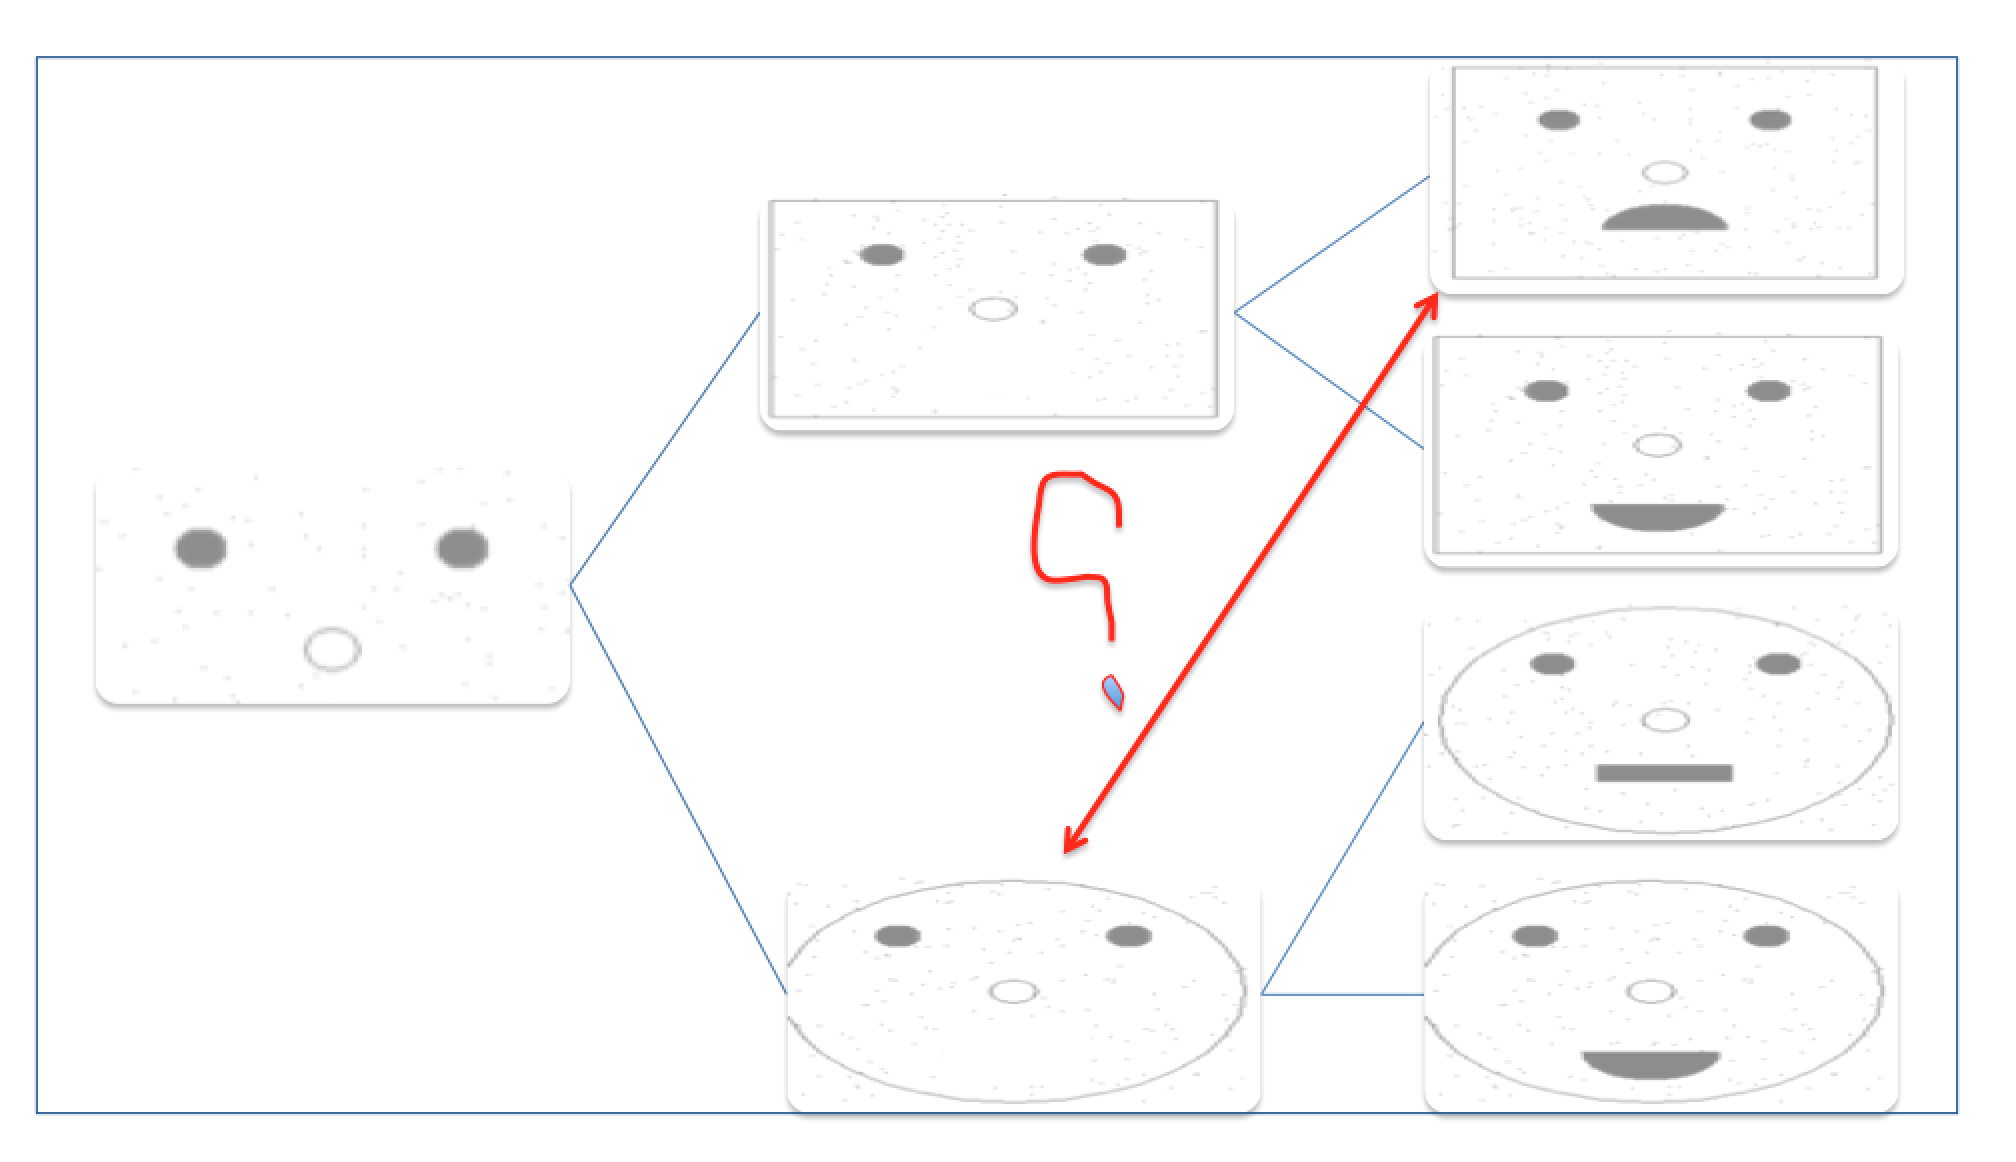
\includegraphics[width=0.8\linewidth]{merge}
 	\end{center}
 	\caption{Example of caption.  It is set in Roman so that mathematics
 		(always set in Roman: $B \sin A = A \sin B$) may be included without an
 		ugly clash.}
 %	\label{fig:long}
 	\label{merge}
 \end{figure}
 
 


 \subsubsection{Fine Grained Data Set}
Due to limited time we just could learn for two hours. We use 10k pixels images for 8 classes and two domains. We reach the accuracy of 70%.

For checking that if one class belong to one of the leaves we compute 
\begin{displaymath}
predictedClass = \operatorname*{arg\,max}_{i \in leaves of Tree} 
\frac{\frac{1}{(1+exp(-\beta'_i.\phi(x)))}}{\|\beta_i\|^2}
\end{displaymath}  

and find the maximum as a desired class.


\begin{figure*}
	\begin{center}
	%	\fbox{\rule{0pt}{2in} \rule{.9\linewidth}{0pt}}
	    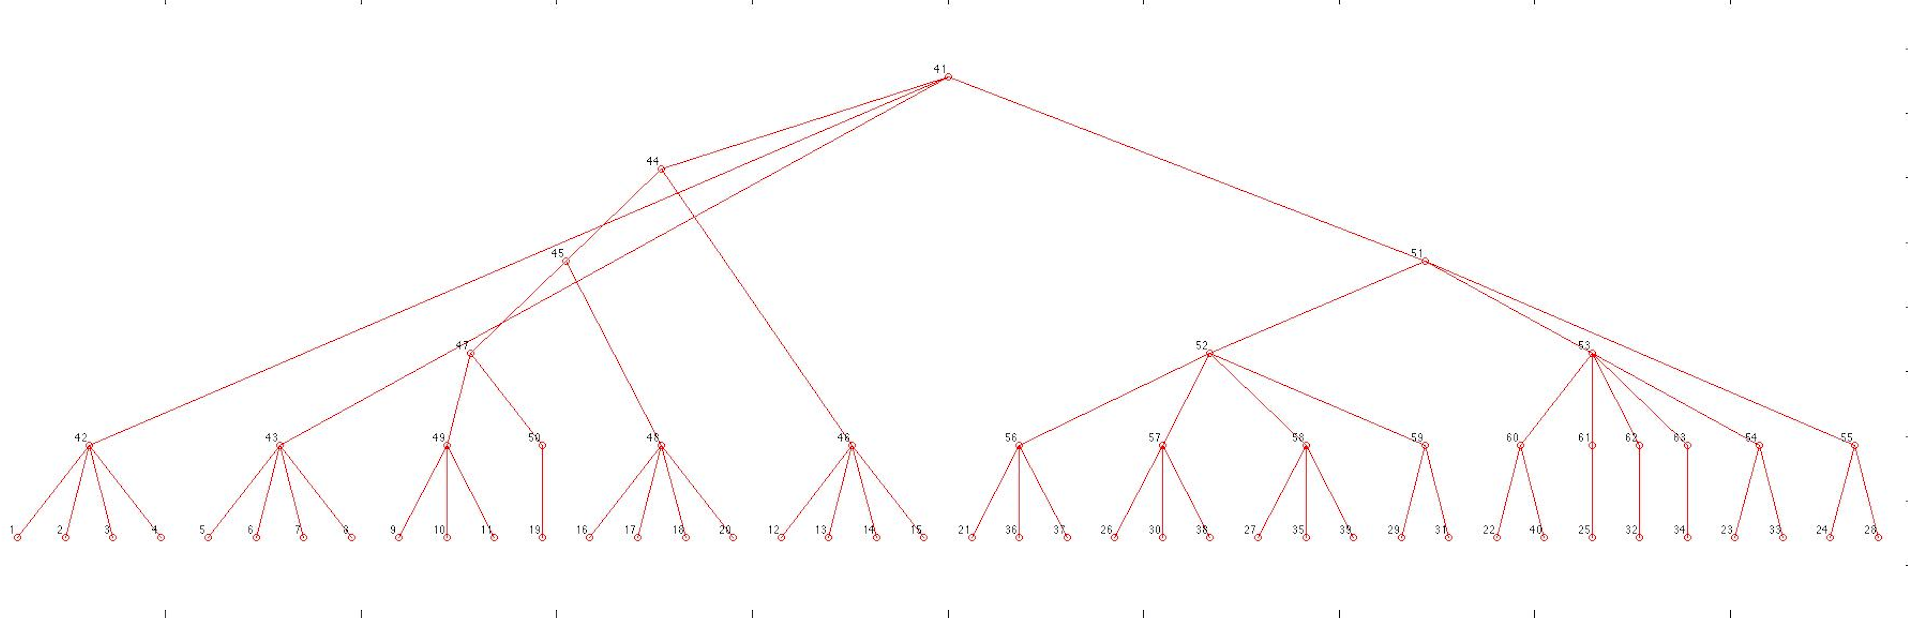
\includegraphics[width=1\linewidth]{carsDogs.png}
	\end{center}
	\caption{Example of a short caption, which should be centered.}
	\label{fig:short}
\end{figure*}
{\small
\bibliographystyle{ieee}
\bibliography{finalReport}
}

\end{document}
